\section{Parallal implementation results}

\begin{frame}{Software ecosystem}
	\begin{tikzpicture}[node distance = 1cm, auto]

	\node [whtblock,text depth=14mm] (FEDDLIB) {
		{\footnotesize \textbf{FEDDLib}\textsuperscript{a}} \\[0.3em] \tiny \textbf{F}inite \textbf{E}lement and \textbf{D}omain \textbf{D}ecomposition \textbf{Lib}rary
		\begin{itemize}
			\item{Parallel finite element assembly}
			\item{Specific problem definition}
			\item{Mesh handling routines}
			      % \item \textcolor{orange}{Update two-level nonlinear Schwarz solver for elasticity and Navier-Stokes}
			      % \item \textcolor{orange}{Test with various coarse spaces}
		\end{itemize}
		% \hspace*{-25mm}\scalebox{.7}{By University of Cologne, TU Delft, TU Freiberg}
	};

	\node [whtblock, right=of FEDDLIB,node distance=7cm, rectangle split part fill={orange!20,blue!5},] (FeatFlow) {
		{ \footnotesize\textbf{FEAT3}\textsuperscript{b}}\\[0.3em] \tiny Finite element based solution of incompressible\\Navier-Stokes in 2D and 3D
		\vspace{2pt}
		\begin{itemize}
			%\setlength{\itemsep}{0pt}
			\item \textcolor{red}{Interface with \texttt{FROSch}}
			\item \textcolor{red}{Test (non-Newtonian, high Reynolds, exascale)}
		\end{itemize}};

	%===============================================    
	\node [whtblock, below=of FEDDLIB, text depth=18mm, node distance=3.5cm,] (Trilinos) {
		{\footnotesize \textbf{Trilinos}\textsuperscript{c}}
		\begingroup
		\addtolength{\leftmargini}{0.5cm}
		\vspace{1pt}
		\tiny
		\begin{itemize}
			%\setlength{\itemsep}{0pt}
			\item Data services: Vectors, matrices, graphs and related operations
			\item Linear and Eigenproblem solvers
			\item Nonlinear solvers and analysis tools
		\end{itemize}
		\endgroup
	};

	\node[inner sep=0pt] (trilinos_logo) at ([xshift=6mm, yshift=0mm] Trilinos.west){
\includegraphics[width=.125\textwidth, angle=90,origin=c]{images/logo/Trilinos_logo_new.png}};

	\node [whtblock, text depth=18mm, right=of Trilinos,node distance=7cm,rectangle split part fill={orange!20,blue!5},] (Frosch) {
		{\footnotesize \textbf{FROSch}\textsuperscript{d}} \\[0.4em]  \hspace{6em}\tiny\textbf{F}ast and \textbf{R}obust \textbf{O}verlapping \textbf{S}chwarz
		\vspace*{0.5em}
		\begingroup
		\addtolength{\leftmargini}{4em}
		\begin{itemize}
			\item \textcolor{red}{Implement two-level nonlinear Schwarz solver}
			\item \textcolor{red}{Test with various coarse spaces on various model problems}
		\end{itemize}
		\endgroup
	};

	\node[inner sep=0pt] (trilinos_logo) at ([xshift=7.5mm, yshift=0mm] Frosch.west){
\includegraphics[width=.1\textwidth]{images/logo/FROSch_logo.png}};

	%%%%%%%%%%%%%%%%%%%%%%%%%%%%%%%%
	%   CONTAINERS -- BACKGROUND LIGHT-DASHED BLOCKS
	%%%%%%%%%%%%%%%%%%%%%%%%%%%%%%%%
	\begin{scope}[on background layer]

		\coordinate (aux2) at ([yshift=0mm]Trilinos.north);
		\node[container2, fit=(aux2) (Trilinos) (Frosch)] (Trilinos_blue) {};

		\coordinate (aux3) at ([yshift=0mm] FeatFlow.north);
		\node[container3, fit=(aux3) (FeatFlow)] (FeatFlow_Green) {};

		\coordinate (aux1) at ([yshift=0mm]FEDDLIB.north);
		\node [container,fit=(aux1) (FEDDLIB)] (FEDDLIB_ORANGE) {};
		\node at ([yshift=0.7mm]Trilinos_blue.north) [fill=gray!10,draw,minimum width=8em,minimum height=1em] (FEDTRI-label) {\footnotesize\textbf{Interface}};

	\end{scope}
	%************************************************************
	%************************************************************
	%  Draw edges
	%************************************************************
	%************************************************************
	% \path [line,thick] (FEDDLIB) -- (FEDTRI-label);
	% \path [line,thick] (Trilinos) -- (Frosch);
	% \path [line,thick] (FEDTRI-label) -- (Trilinos);
	% \path [line,red,thick] (FeatFlow) -- (FEDTRI-label);

\end{tikzpicture}
\tiny\\~\\

a: University of Cologne, TU Delft, TU Freiberg (https://github.com/FEDDLib/FEDDLib.git)\\
b: TU Dortmund (https://github.com/tudo-math-ls3/feat3)\\
c: Sandia National Laboratories (https://trilinos.github.io)\\
d: University of Cologne, TU Delft, TU Freiberg (https://shylu-frosch.github.io)\\

\end{frame}

\begin{frame}{Stationary and dimensionless Navier-Stokes equations}
	\vspace{-5mm}
	\begin{columns}
		\begin{column}{0.6\textwidth}%
			\begin{align*}
				-\frac{1}{Re} \Delta v + (v \cdot \nabla)v + \nabla p & = 0 \;   & {\rm in}\; \Omega           \\
				{\rm div}(v)                                          & = 0 \;   & {\rm in} \; \Omega          \\
				v                                                     & = v_0 \; & {\rm on} \; \partial \Omega
			\end{align*}
			\vspace{-4mm}
			\begin{itemize}
				\item $v_0=(1,0)$ on the lid and zero everywhere else
				\item $P_1\textrm{-}P_1\textrm{-}Stab$ (Bochev-Dohrmann) \footnotemark{}
				\item Subdomain size: $150\times 150$ elements
				\item Solver absolute and relative tolerances: \num{e-6}
        \item RGDSW coarse space \footnotemark[6]$^,$\footnotemark[7]$^,$\footnotemark[8]$^,$\footnotemark[9]$^,$\footnotemark[10]
                \item Hybrid variant
			\end{itemize}
		\end{column}
		\begin{column}{0.4\textwidth}
			\begin{figure}
				\centering
				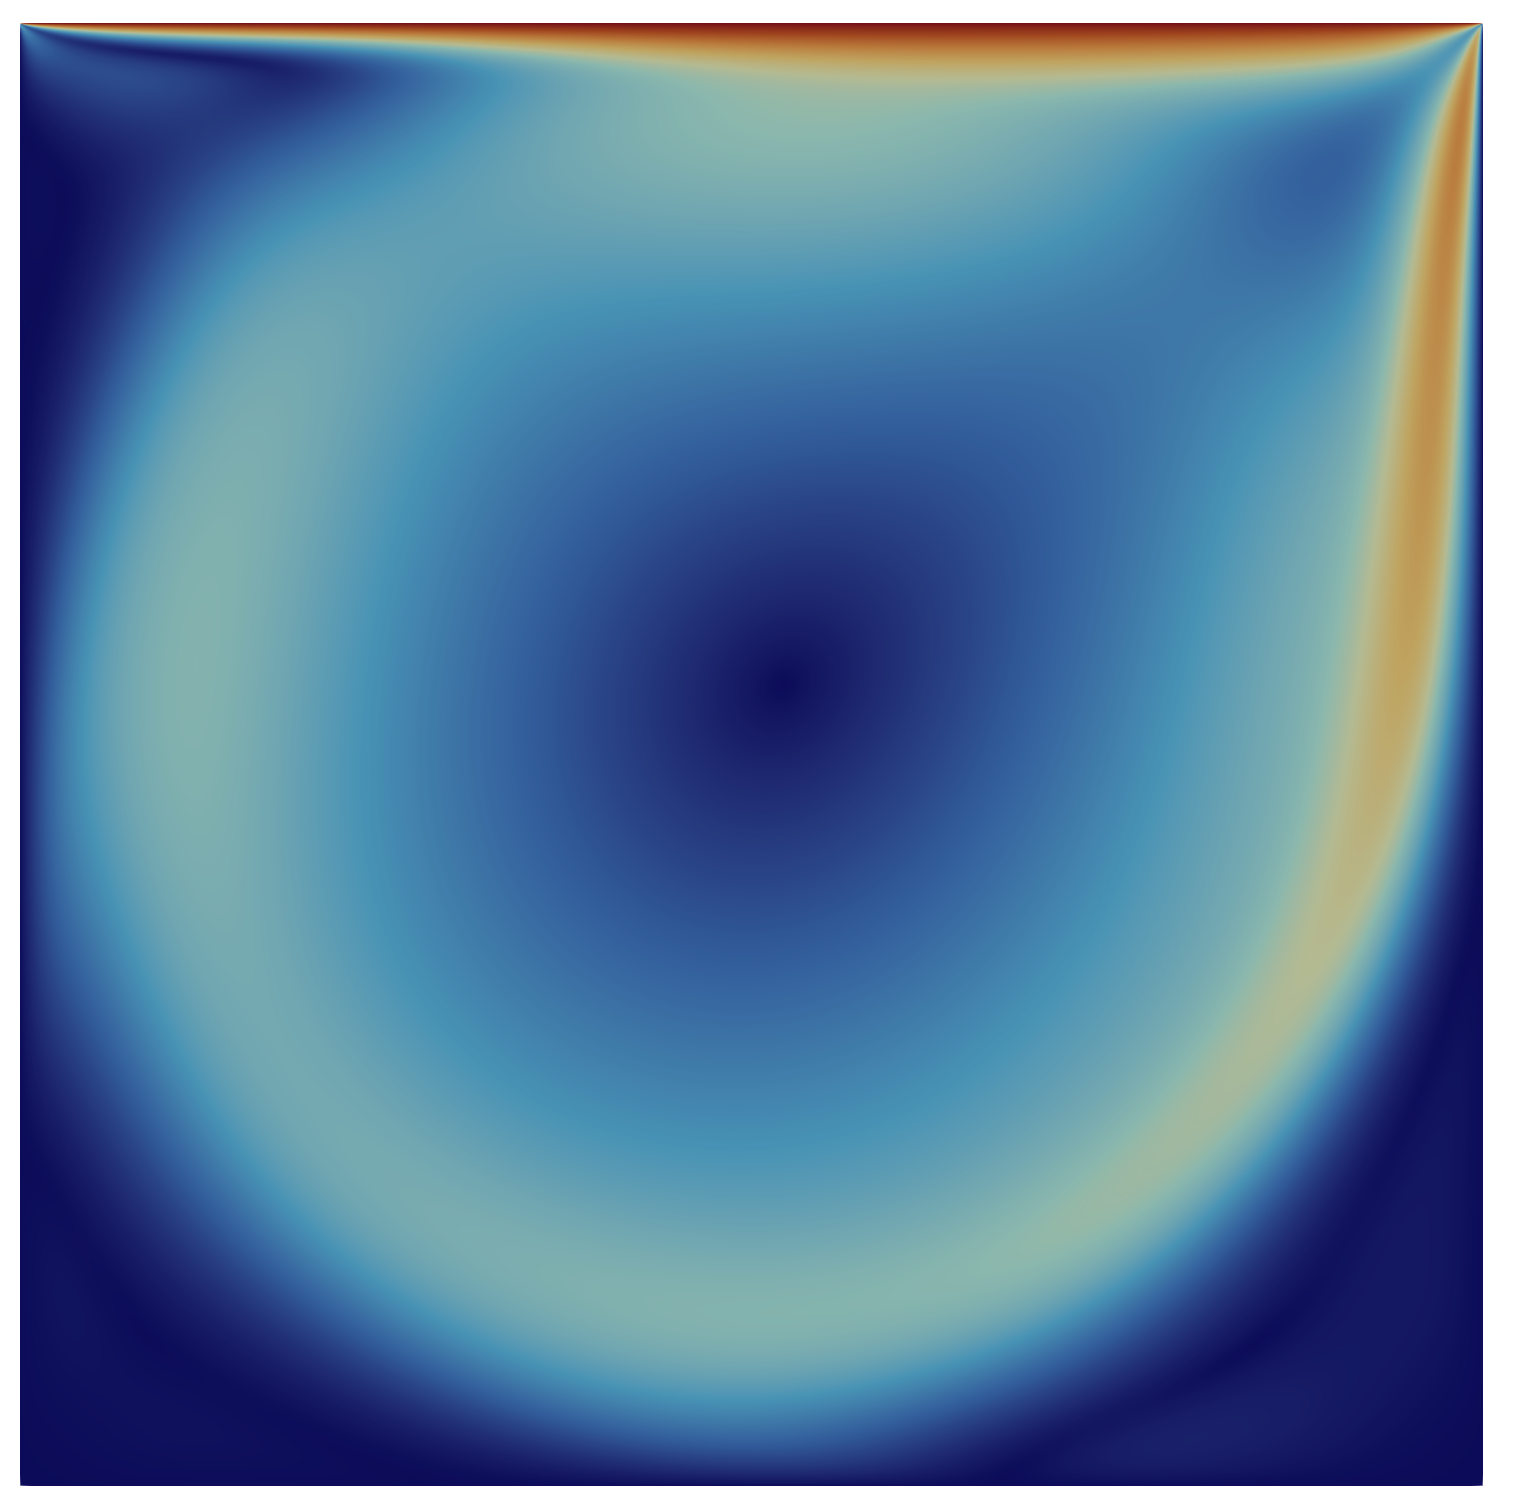
\includegraphics[width=0.7\textwidth]{images/ldc.png}
				\caption{Lid-driven cavity}
			\end{figure}
		\end{column}
	\end{columns}
    {\let\thefootnote\relax\footnote{{\tiny \textsuperscript{5}Bochev, Dohrmann (2004),  \textsuperscript{6}Dohrmann, Widlund (2017), \textsuperscript{7}Heinlein, Hochmuth, Klawonn (2020),  \textsuperscript{8}Disstertation Hochmuth (2021),\\\hspace{3em}\textsuperscript{9}Lanser, Klawonn (2024),  \textsuperscript{10}Heinlein, Klawonn, Knepper, Saßmannshausen (2025)}}}
\end{frame}

\begin{frame}{Lid-driven cavity: nonlinear Schwarz weak scalability}
	\begin{figure}
		\centering
		\begin{tikzpicture}
	\pgfplotsset{
		every axis/.append style={
				ybar stacked,
				width=13cm,
				height=7cm,
				ylabel={Runtime (seconds)},
				xlabel={Num. subdomains},
				symbolic x coords={256, 576, 1024, 2025, 4096, 9216},
				xtick=data,
				enlarge x limits=0.15,
				legend style={at={(1,1)},anchor=north west},
				axis lines*=left, ymajorgrids, yminorgrids,
				ymin=0,
				ymax=250,
				bar width=8pt,
				minor y tick num=1,
				xticklabel style={rotate=0,xshift=0ex,anchor=north},
				cycle list name=Set2-5,
			},
		% Ensures that bars are plotted full
		every axis plot/.append style={
				fill,
			},
	}
  \tikzstyle{mynodestyle} = [rotate=90, anchor=west]

	% Re = 1000
	\begin{axis}[bar shift=-11pt, hide axis]
		% Another option for relative node placement
		% \node [left=11pt of 256.base, anchor=base] {test}; % Custom number above bar for 256
		\node[mynodestyle] (one) at ([xshift=-11pt]axis cs:256,105) {$450$ $(4)$};
		\node[mynodestyle] at ([xshift=-11pt]axis cs:576,105) {$390$ $(4)$};
		\node[mynodestyle] at ([xshift=-11pt]axis cs:1024,83){$240$ $(3)$};
		\node[mynodestyle] at ([xshift=-11pt]axis cs:2025,85){$210$ $(3)$};
		\node[mynodestyle] at ([xshift=-11pt]axis cs:4096,85){$180$ $(3)$};
		\node[mynodestyle] at ([xshift=-11pt]axis cs:9216,105){$220$ $(4)$};
		\node (oneRe) at ([xshift=-11pt]axis cs:9216,15) {$1$};

        \addplot coordinates  {(256,23.8 ) (576,  22.8 ) (1024, 18.3 ) (2025, 20	) (4096, 17.9)  (9216,22.6  )};   
        \addplot+ coordinates {(256,18.3 ) (576,  19.9 ) (1024, 19.8 ) (2025, 22	) (4096, 25.9)  (9216,31.3)}; 
        \addplot+ coordinates {(256,42.2 ) (576,  40.3 ) (1024, 25 )   (2025, 22.8	) (4096, 20.7)  (9216,25.5)};   
        \addplot+ coordinates {(256,23.7 ) (576,  26   ) (1024, 22.8 ) (2025, 23.9	) (4096, 24.1)  (9216,29.6)}; 







    \end{axis}

	% Re = 2000
	\begin{axis}[bar shift=0pt, hide axis]

		\node[rotate=0] at (axis cs:256,12) {\scriptsize\color{red}\ding{55}};
		\node[mynodestyle](576) at (axis cs:576,155) {$610$ $(5)$};
		\node[mynodestyle](1024) at (axis cs:1024,120) {$440$ $(4)$};
		\node[mynodestyle](2025) at (axis cs:2025,123) {$370$ $(4)$};
		\node[mynodestyle](4096) at (axis cs:4096,120) {$310$ $(4)$};
		\node[mynodestyle](9216) at (axis cs:9216,115) {$240$ $(4)$};
		\node at (axis cs:9216,15) {$2$};


        \addplot coordinates  {(256, 0)     (576,32.1) (1024, 25.2) (2025, 25.8) (4096, 24.8)  (9216,24  )};
        \addplot+ coordinates {(256, 0)     (576,26.4) (1024, 23.4) (2025, 28.7) (4096, 31.7)  (9216,34.5)};
        \addplot+ coordinates {(256, 0)     (576,66.4) (1024, 46  ) (2025, 40.7) (4096, 36.1)  (9216,29.4  )};
        \addplot+ coordinates {(256, 0)     (576,30.7) (1024, 26.8) (2025, 28.8) (4096, 29.4)  (9216,29.1)};
	\end{axis}

	% Re = 4000
	\begin{axis}[bar shift=11pt]

		\node[xshift=11pt,rotate=0] at (axis cs:256,12) {\scriptsize\color{red}\ding{55}};
		\node[xshift=11pt,rotate=0] at (axis cs:576,12) {\scriptsize\color{red}\ding{55}};
		\node[xshift=11pt,rotate=0] at (axis cs:1024,12) {\scriptsize\color{red}\ding{55}};
		\node [mynodestyle]at([xshift=11pt]axis cs:2025,178) {$620$ $(5)$};
		\node [mynodestyle]at([xshift=11pt]axis cs:4096,135) {$400$ $(4)$};
		\node [mynodestyle]at([xshift=11pt]axis cs:9216,127) {$340$ $(4)$};
		\node(fourRe) at ([xshift=11pt]axis cs:9216,15) {$4$};

        \addplot+ coordinates { (256, 0) (576, 0) (1024, 0) (2025,33.8) (4096,26.6) (9216,24.4)}; 
        \addplot+ coordinates { (256, 0) (576, 0) (1024, 0) (2025,39)  (4096,31.7)  (9216,35.7)};   
        \addplot+ coordinates { (256, 0) (576, 0) (1024, 0) (2025,72.5) (4096,50)   (9216,41.4)};  
        \addplot+ coordinates { (256, 0) (576, 0) (1024, 0) (2025,34.7) (4096,29.7) (9216,28.5)}; 

    \node[anchor=south,text width=1.6cm] (gmres) at (axis cs:256,180){GMRES its. (Newton its.)};

		\legend{
			Inner solve,
			Coarse solve,
			GMRES,
			Other
		}

	\end{axis}

	\node[rotate=0, text width=1.8cm] (Re) at ([yshift=-5,xshift=50]fourRe){Re ($\times 10^{3}$)};

	% \draw [thin] (gmres) --  (256);
	\draw [thin] (gmres) --  (one);
	% \draw [thin] (gmres) --  (three);

	\draw [thin] (Re) --  (fourRe);

\end{tikzpicture}

		\label{fig:weak-scalability-nls}
	\end{figure}
\end{frame}

\begin{frame}{Lid-driven cavity: nonlinear Schwarz weak scalability}
	\begin{figure}
		\centering
		\begin{tikzpicture}
	\pgfplotsset{
		every axis/.append style={
				ybar stacked,
				width=13cm,
				height=7cm,
				ylabel={Avg. runtime per iter. (seconds)},
				xlabel={Num. subdomains},
				symbolic x coords={256, 576, 1024, 2025, 4096, 9216},
				xtick=data,
				enlarge x limits=0.15,
				legend style={at={(0,1)},anchor=north west},
				axis lines*=left, ymajorgrids,
				ymin=0,
				ymax=55,
				bar width=8pt,
				nodes near coords,
				nodes near coords style={rotate=90},
				minor y tick num=1,
				xticklabel style={rotate=0,xshift=0ex,anchor=north},
				cycle list name=Set2-5,
			},
		% Ensures that bars are plotted full
		every axis plot/.append style={
				fill,
				% fill opacity=0.5,
				every node/.append style={
						text=black,
					},
			},
	}
	% Re = 1000

	\begin{axis}[bar shift=-11pt, hide axis]
		\addplot+ coordinates {(256,5.9  ) (576, 5.7	 ) (1024,   6.1) (2025,  6.7 ) (4096, 6) (9216,5.7 )};
		\addplot+ coordinates {(256,4.6 ) (576, 5 )  (1024,  6.6 ) (2025,  7.3 ) (4096, 8.6 )    (9216,7.8)};
		\addplot+ coordinates {(256,10.6 ) (576, 10.1)  (1024,  8.3 ) (2025,  7.6 ) (4096, 6.9 ) (9216,6.4  )};
		\addplot+ coordinates {(256,5.9 ) (576, 6.5	 ) (1024,   7.6) (2025,  8) (4096, 8   )     (9216,7.4 )};
	\end{axis}

	% Re = 2000
	\begin{axis}[bar shift=0pt, hide axis]

		\node[rotate=0] at (axis cs:256,2) {\scriptsize\color{red}\ding{55}};
		\addplot+ coordinates {(256, 0) (576,6.4 ) (1024, 6.3	) (2025,  6.5   )  (4096,  6.2   ) (9216,6   )};
		\addplot+ coordinates {(256, 0) (576,5.3 ) (1024, 5.9  ) (2025,  7.2  ) (4096,  7.9 )      (9216,8.6)};
		\addplot+ coordinates {(256, 0) (576,13.3) (1024, 11.5  ) (2025,  10.2 ) (4096,  9 )       (9216,7.4  )};
		\addplot+ coordinates {(256, 0) (576,6.1 ) (1024, 6.7	) (2025,  7.2	 )  (4096,  7.3  ) (9216,7.3)};
	\end{axis}

	% Re = 4000
	\begin{axis}[bar shift=11pt]

		\node[xshift=11pt,rotate=0] at (axis cs:256,2) {\scriptsize\color{red}\ding{55}};
		\node[xshift=11pt,rotate=0] at (axis cs:576,2) {\scriptsize\color{red}\ding{55}};
		\node[xshift=11pt,rotate=0] at (axis cs:1024,2) {\scriptsize\color{red}\ding{55}};

		\addplot+ coordinates {(256,0) (576,0) (1024,0)  (2025,  6.8) (4096, 6.7  )   (9216,6.1 )};
		\addplot+ coordinates {(256,0) (576,0) (1024,0)  (2025,  7.8 ) (4096, 7.9)    (9216,8.9  )};
		\addplot+ coordinates {(256,0) (576,0) (1024,0)  (2025,  14.5) (4096, 12.5  ) (9216,10.4)};
		\addplot+ coordinates {(256,0) (576,0) (1024,0)  (2025,  6.9) (4096, 7.4)     (9216,7.1)};

		\legend{
			Inner solve,
			Coarse solve,
			GMRES,
			Other
		}
	\end{axis}
\end{tikzpicture}

		\label{fig:weak-scalability-per-iter-nls}
	\end{figure}
\end{frame}

\begin{frame}{Lid-driven cavity: Newton-Krylov-Schwarz vs Hybrid}
	\begin{itemize}
		\item $256$ subdomains
	\end{itemize}
	\begin{figure}
		\centering
		\begin{tikzpicture}
    \begin{groupplot}[
        group style={group size=1 by 2, vertical sep=1.cm},
        width=13cm, height=4cm,
        xlabel={Iter.},
        grid=major,
        log basis y=10,
        legend style={at={(1.0,0.9)},anchor=east},
				xmin=0,
				xmax=15,
				ymin=1e-6,
				ymax=1,
        every axis plot/.append style={line width=1pt, mark size=1.5pt, mark=*},
    ]
    \nextgroupplot[
        ylabel={Rel. residual},
        ymode=log,
    ]
    \addplot coordinates {
        (0, 1) (1, 0.00320133) (2, 0.00143493) (3, 0.000610389) 
        (4, 0.000369944) (5, 0.000215426) (6, 1.11767e-05) (7, 4.18693e-08)
    };
    \addlegendentry{Re=500}
    \addplot coordinates {
        (0, 1) (1, 0.00480191) (2, 0.00380737) (3, 0.00297334)
        (4, 0.00272655) (5, 0.00272013) (6, 0.00270843) (7, 0.00268613)
        (8, 0.00267774) (9, 0.00266959) (10, 0.00243689) (11, 0.0024165)
        (12, 0.00223072) (13, 0.00221035) (14, 0.002201) (15, 0.00219758)
        (16, 0.00219347) (17, 0.00219139) (18, 0.00219044) (19, 0.00219027)
        (20, 0.00218816) (21, 0.00218768) (22, 0.0021868) (23, 0.00218531)
        (24, 0.00218251) (25, 0.00217408) (26, 0.00217307) (27, 0.00217296)
        (28, 0.00217293) (29, 0.00217293)
    };
    \addlegendentry{Re=750}
    \addplot coordinates {
        (0, 1) (1, 0.00640242) (2, 0.00404174) (3, 0.00228814)
        (4, 0.00160117) (5, 0.00132757) (6, 0.00119772) (7, 0.00119687)
        (8, 0.00119643) (9, 0.00119643) (10, 0.00119643) (11, 0.00119643)
        (12, 0.00119643) (13, 0.00119643) (14, 0.00119643) (15, 0.00119643)
        (16, 0.00119643) (17, 0.00119643) (18, 0.00119643) (19, 0.00119643)
        (20, 0.00119643) (21, 0.00119643) (22, 0.00119643) (23, 0.00119643)
        (24, 0.00119643) (25, 0.00119643) (26, 0.00119643) (27, 0.00119643)
        (28, 0.00119643) (29, 0.00119643)
    };
    \addlegendentry{Re=1000}


    % Absolute residual plot
    \nextgroupplot[
        ylabel={Rel. residual},
        ymode=log,
    ]
    \addplot coordinates {
        (0, 1) (1, 0.0216039) (2, 0.00240872) (3, 3.08805e-05) (4, 5.87615e-07)
    };
    \addlegendentry{$Re=500$}

    \addplot coordinates {
        (0, 1) (1, 0.0410675) (2, 0.00701551) (3, 8.12889e-05) (4, 5.1786e-07)
    };
    \addlegendentry{$Re=750$}

    % \pgfplotsset{cycle list shift=1}
    \addplot coordinates {
        (0, 1) (1, 0.0635524) (2, 0.0125035) (3, 0.000197537) (4, 1.25259e-06)
    };
    \addlegendentry{$Re=1000$}

    \addplot coordinates {
        (0, 1) (1, 0.10807) (2, 0.0229372) (3, 0.0025968) (4, 0.00019946) (5, 7.0061e-07)
    };
    \addlegendentry{$Re=1500$}
    \end{groupplot}
\end{tikzpicture}

		\label{fig:residual-ldc-256}
	\end{figure}
\end{frame}

\begin{frame}{Lid-driven cavity: Newton-Krylov-Schwarz vs Hybrid}
	\begin{itemize}
		\item $256$ subdomains
	\end{itemize}
	\begin{figure}
		\centering
		\begin{tikzpicture}
	\begin{groupplot}[
			group style={group size=1 by 2, vertical sep=1.5cm},
			width=13cm, height=3.8cm,
			xlabel={Iter.},
			grid=major,
			log basis y=10,
			legend style={at={(1.0,0.9)},anchor=east},
			xmin=0,
			xmax=15,
			ymin=1e-6,
			ymax=1,
			every axis plot/.append style={line width=1pt, mark size=1.5pt, mark=*},
		]
		\nextgroupplot[
			ylabel={Rel. residual},
            title={\bf{Newton-Krylov-Schwarz}},
			ymode=log,
		]
		\addplot coordinates {
				(0, 1) (1, 0.000461063) (2, 0.000180623) (3, 7.69231e-05) (4, 4.67144e-05) (5, 2.75539e-05) (6, 1.50771e-06) (7, 6.3394e-09)
			};
		\addlegendentry{Re=500}
		\addplot coordinates {
				(0, 1) (1, 0.000683264) (2, 0.000480095) (3, 0.00037343) (4, 0.000345118) (5, 0.000341495) (6, 0.000339957) (7, 0.000339534) (8, 0.000414796) (9, 0.000364827) (10, 0.000333536) (11, 0.000317937) (12, 0.000275248) (13, 0.000256005) (14, 0.000254507) (15, 0.000254237) (16, 0.000262081) (17, 0.00025798) (18, 0.000261379) (19, 0.000260608)
			};
		\addlegendentry{Re=750}
		\addplot coordinates {
            (0, 1) (1, 0.000907096) (2, 0.000549946) (3, 0.000287238) (4, 0.000198314) (5, 0.000160798) (6, 0.000151072) (7, 0.000150393) (8, 0.000150489) (9, 0.000155954) (10, 0.000154682) (11, 0.000154337) (12, 0.000159684) (13, 0.000159413) (14, 0.000172403) (15, 0.000172074) (16, 0.000172708) (17, 0.000189149) (18, 0.000190431) (19, 0.000198664) 
			};
		\addlegendentry{Re=1000}


		% Absolute residual plot
		\nextgroupplot[
			ylabel={Rel. residual},
            title={\bf{Hybrid Nonlinear Schwarz}},
			ymode=log,
		]
		\addplot coordinates {
				(0, 1) (1, 0.00361003) (2, 4.0282e-05) (3, 9.87625e-07)
			};
		\addlegendentry{$Re=500$}

		\pgfplotsset{cycle list shift=1}
		\addplot coordinates {
				(0, 1) (1, 0.0783692) (2, 0.00100882) (3, 2.29151e-06)
			};
		\addlegendentry{$Re=1000$}

		\pgfplotsset{cycle list shift=1}
		\addplot coordinates {
				(0, 1) (1, 0.0436383) (2, 0.00622051) (3, 6.42127e-05) (4, 9.38152e-07)
			};
		\addlegendentry{$Re=3000$}

		\addplot coordinates {
				(0, 1) (1, 0.0994514) (2, 0.0140707) (3, 0.00294689) (4, 0.000409486) (5, 1.93227e-05)
			};
		\addlegendentry{$Re=6000$}
	\end{groupplot}
\end{tikzpicture}

		\label{fig:residual-ldc-4096}
	\end{figure}
\end{frame}

\begin{frame}{LDC coarse basis functions}
	\begin{figure}
		\centering
		\begin{subfigure}{0.5\textwidth}
			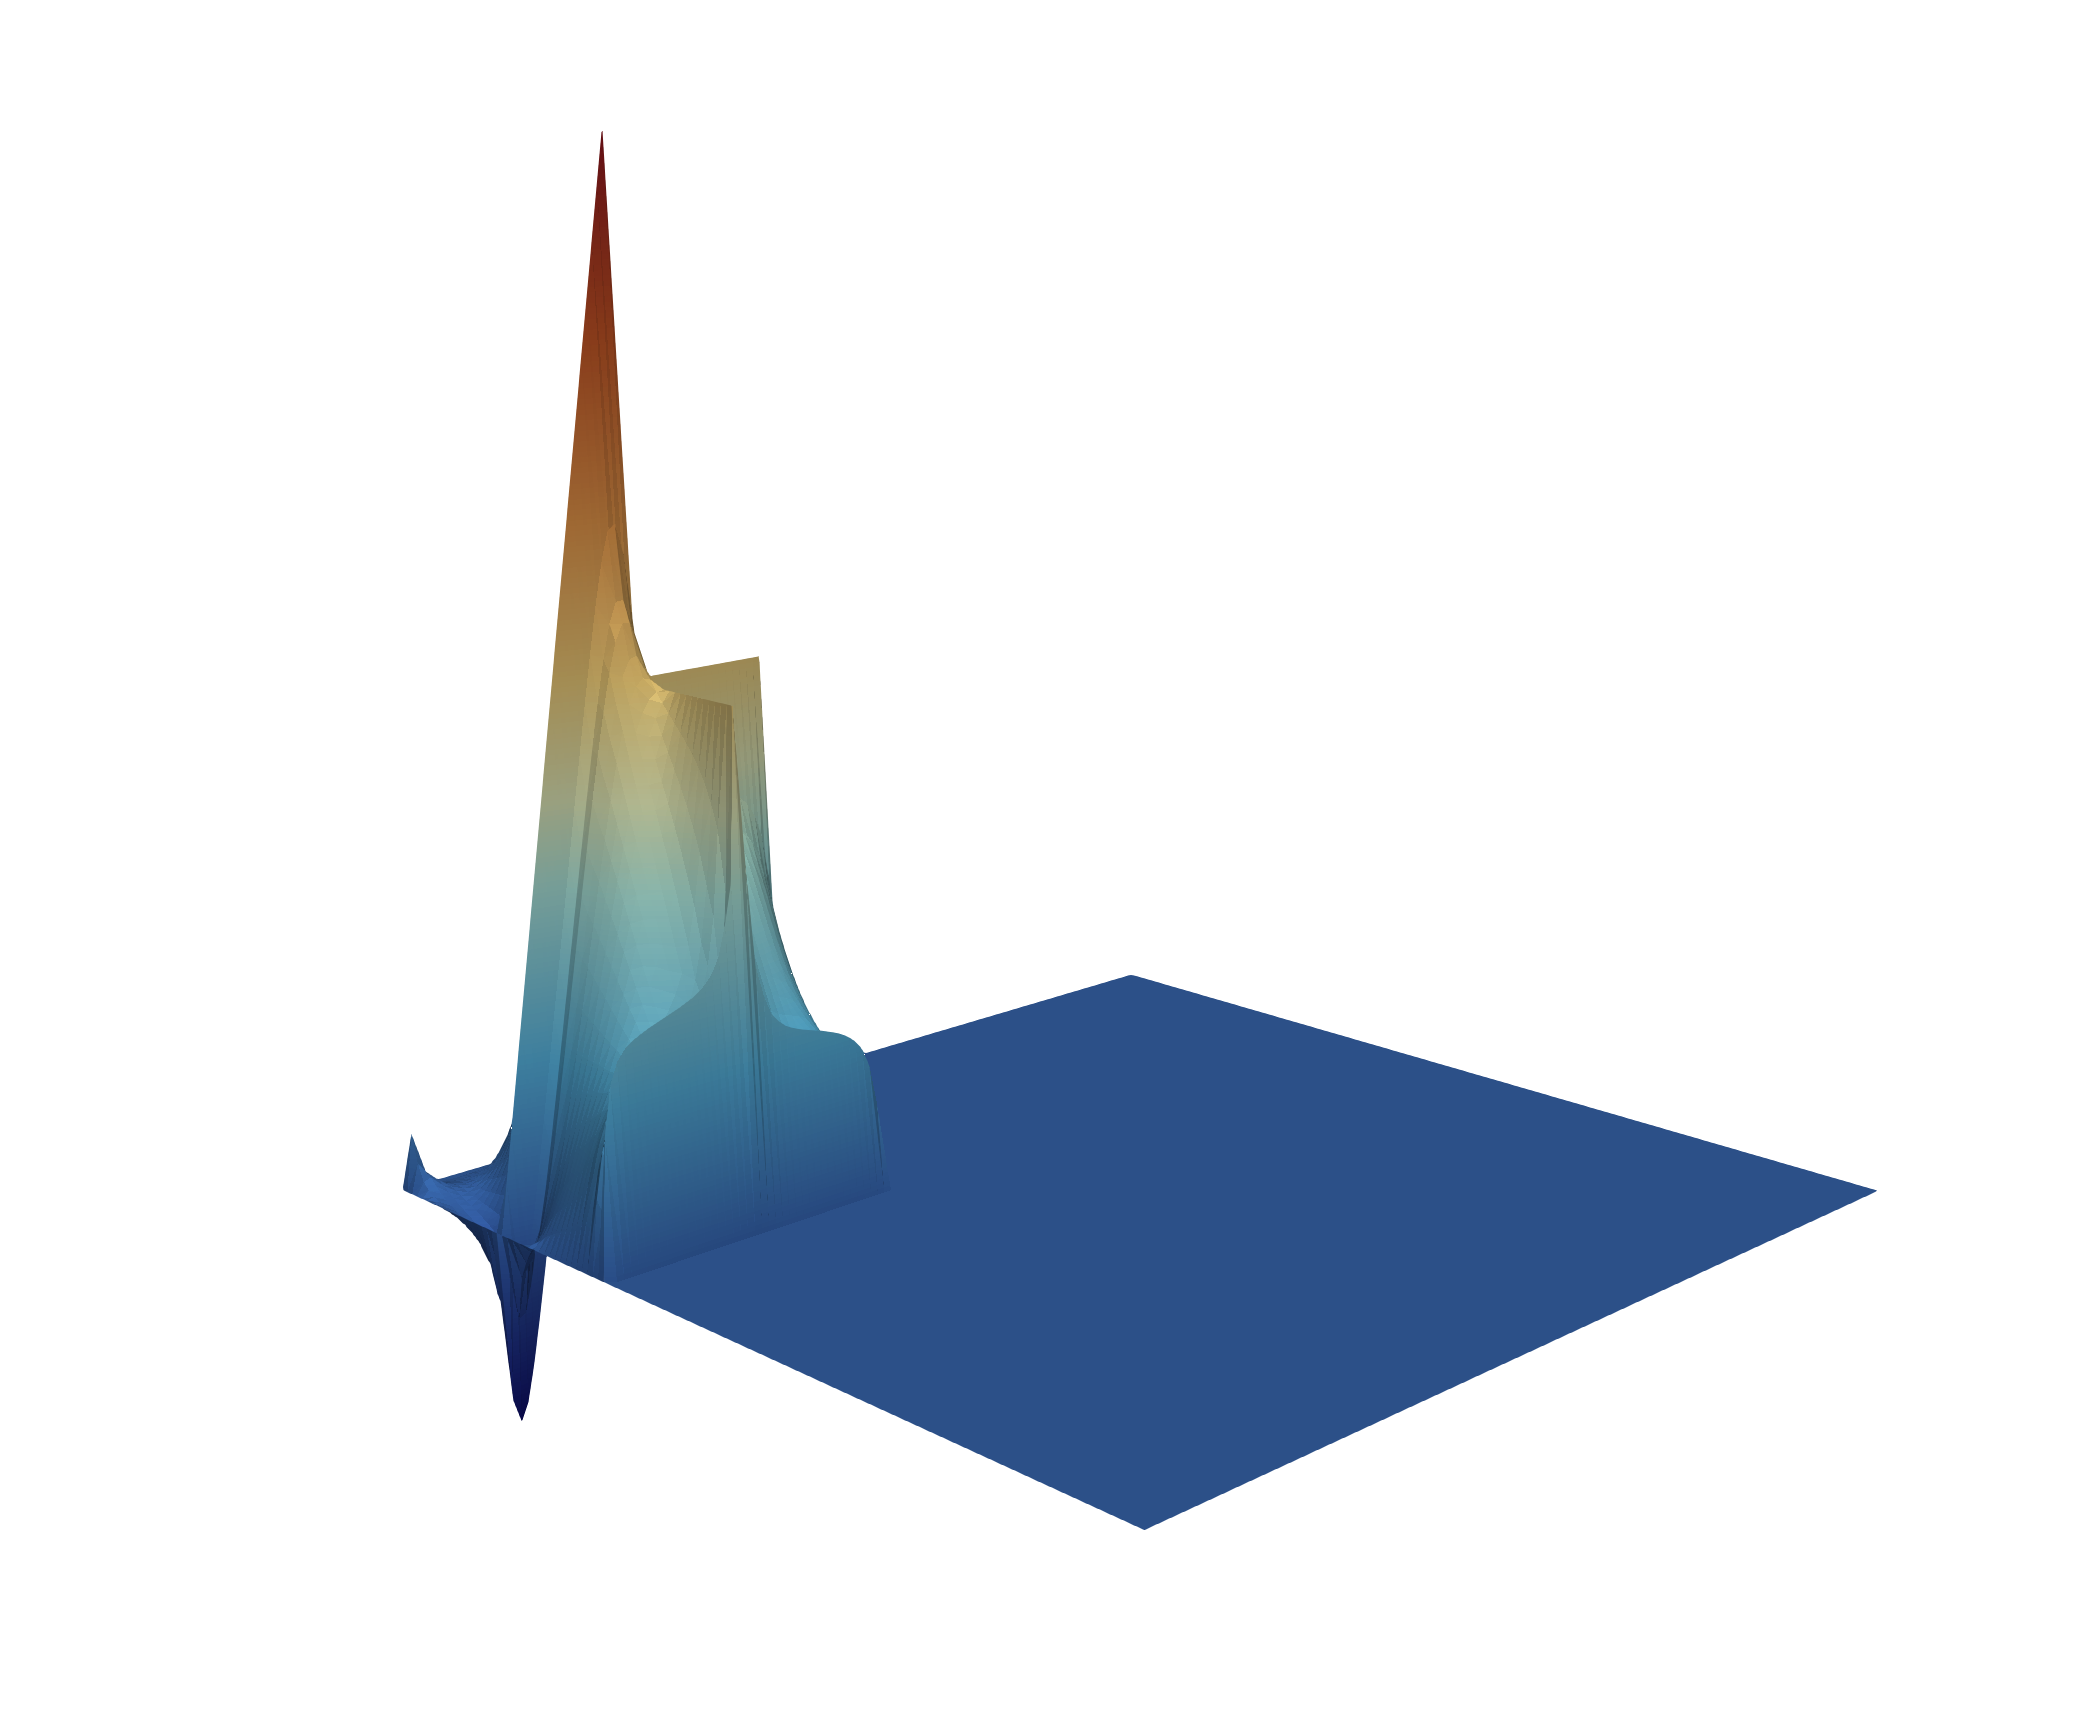
\includegraphics[width=\textwidth]{images/RGDSW-x}
			\caption{RGDSW $x$ component.}
		\end{subfigure}%
		\begin{subfigure}{0.5\textwidth}
			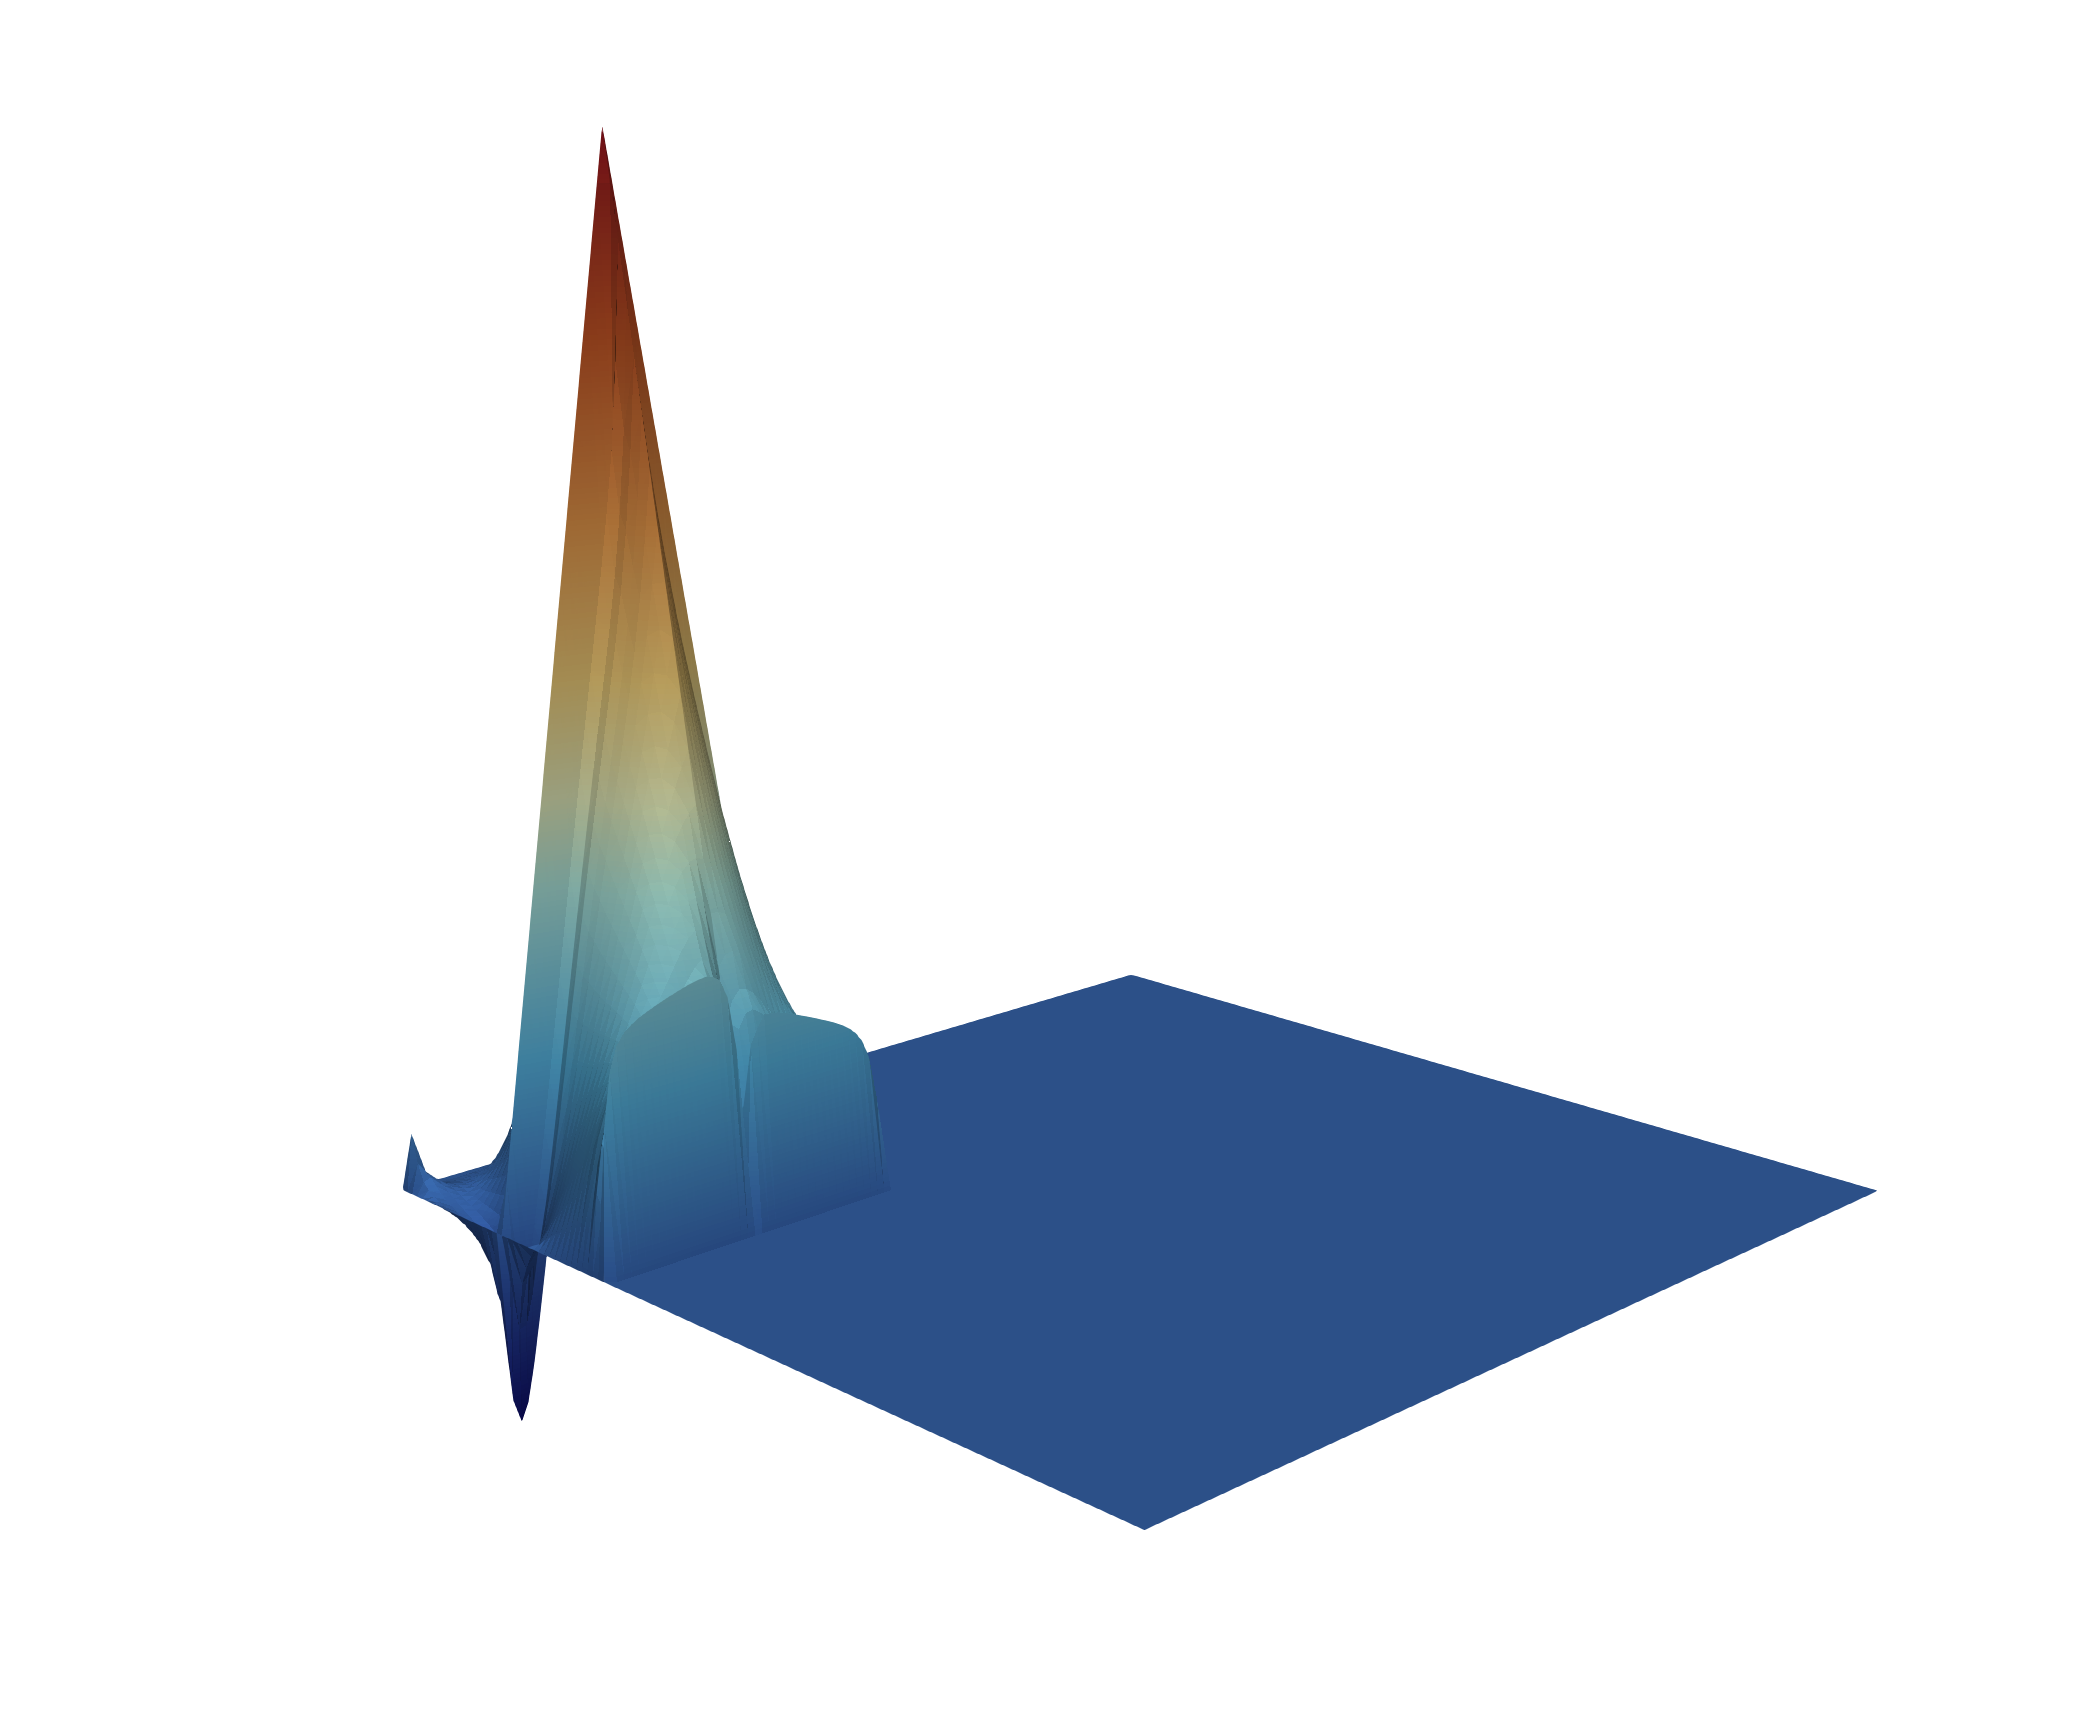
\includegraphics[width=\textwidth]{images/MsFEM-x}
			\caption{MsFEM $x$ component.}
		\end{subfigure}
		\caption{Components of $x$ velocity coarse basis function.}
	\end{figure}
\end{frame}

\begin{frame}{MsFEM vs. RGDSW}
	% Mention that: 
	%   - Re has no effect 
	%   - MsFEM was faster for Re=1000 but maybe RGDSW can be sped up with proper tuning
	%   - These results were generated with higher GMRES tollerance which increases GMRES count and runtime without a positive effect
	\begin{itemize}
		\item $256$ subdomains
	\end{itemize}
	\begin{figure}
		\centering
		\begin{tikzpicture}
	\pgfplotsset{
		every axis/.append style={
				ybar stacked,
				width=13cm,
				height=7cm,
				ylabel={Runtime (seconds)},
				xlabel={$Re$},
				symbolic x coords={500, 750, 1000, 1500, 2000},
				xtick=data,
				enlarge x limits=0.15,
				legend style={at={(0.9,1)},anchor=north west},
				axis lines*=left, ymajorgrids, yminorgrids,
				ymin=0,
				ymax=175,
				bar width=12pt,
				minor y tick num=1,
				xticklabel style={rotate=0,xshift=0ex,anchor=north},
				cycle list name=Set2-5,
			},
		% Ensures that bars are plotted full
		every axis plot/.append style={
				fill,
			},
	}
	% RGDSW
	\begin{axis}[bar shift=-8pt, hide axis]
		\node [rotate=90](rgdsw) at ([xshift=-8pt]axis cs:500,15) {RGDSW};
		% Inner solve
		\addplot coordinates {(500,22) (750,23.7) (1000,23.8) (1500,31) (2000,0)};
		% Coarse solve
		\addplot coordinates {(500,17.4) (750,17.1) (1000,18.3) (1500,24) (2000,0)};
		% GMRES
		\addplot coordinates {(500,28.6) (750,37) (1000,42.2) (1500,64) (2000,0)};
		% Other
		\addplot coordinates {(500,23.7) (750,22.6) (1000,23.7) (1500,28) (2000,0)};

		\node [rotate=90,anchor=center](500) at ([xshift=-8pt]axis cs:500,105) {$320$ $(4)$};
		\node [rotate=90,anchor=center](750) at ([xshift=-8pt]axis cs:750,113) {$400$ $(4)$};
		\node [rotate=90,anchor=center](1000) at ([xshift=-8pt]axis cs:1000,122) {$450$ $(4)$};
		\node [rotate=90,anchor=center](1500) at ([xshift=-8pt]axis cs:1500,160) {$650$ $(5)$};
		\node at ([xshift=-8pt]axis cs:2000,6) {\scriptsize\color{red}\ding{55}};

	\end{axis}

	\begin{axis}[bar shift=8pt]
		\node [rotate=90](msfem) at ([xshift=8pt]axis cs:500,15) {MsFEM};
		% Inner solve
		\addplot coordinates {(500,21.9) (750,21.9) (1000,0) (1500,0) (2000,0)};
		% Coarse solve                            
		\addplot coordinates {(500,22.3) (750,24  ) (1000,0) (1500,0) (2000,0)};
		% GMRES                                   
		\addplot coordinates {(500,25.6) (750,28.9) (1000,0) (1500,0) (2000,0)};
		% Other                                   
		\addplot coordinates {(500,23.7) (750,23.9) (1000,0) (1500,0) (2000,0)};


		\legend{
			Inner solve,
			Coarse solve,
			GMRES,
			Other
		}
		\node[rotate=90,anchor=center](one) at ([xshift=8pt]axis cs:500,107) {$300$ $(4)$};
		\node[rotate=90,anchor=center] at ([xshift=8pt]axis cs:750,112) {$330$ $(4)$};

		\node at ([xshift=8pt]axis cs:1000,6) {\scriptsize\color{red}\ding{55}};
		\node at ([xshift=8pt]axis cs:1500,6) {\scriptsize\color{red}\ding{55}};
		\node at ([xshift=8pt]axis cs:2000,6) {\scriptsize\color{red}\ding{55}};


	\end{axis}

	\node[rotate=0, text width=1.6cm] (gmres) at ([xshift=8,yshift=40]500){GMRES its. (Newton its.)};
	% \node[rotate=0, text width=1.8cm] (coarsespace) at ([yshift=-60,xshift=-10]1000){Coarse space};

	\draw [thin] (gmres) --  (500);
	\draw [thin] (gmres) --  (one);

	% \draw [thin] (coarsespace) --  (rgdsw);
	% \draw [thin] (coarsespace) --  (msfem);

\end{tikzpicture}

		\label{fig:msfem-vs-rgdsw}
	\end{figure}
\end{frame}

\begin{frame}{Summary lid-driven cavity}
	\begin{itemize}
		\item Hybrid more robust than NKS against nonlinearity
		\item It's weak scaling is excellent up to $4096$ subdomains\\then coarse solve time increases % (larger coarse space improves nonlinear preconditioning)
		\item It's difficult to tune e.g. what makes a good coarse space?%: many parameters that have a potentialy significant impact on performance
	\end{itemize}

    \begin{center}
        \includegraphics[width=0.5\textwidth]{images/nls.png}\\
        {\tiny \vspace{-2mm}\hspace{-4.7cm}Generated with ChatGPT}
    \end{center}
	% Bottom line: very sensitive to proper tuning, The coarse space does not encode the Re somehow but it's discretisation properties are critical.
\end{frame}



